\documentclass[10pt, a4paper]{scrartcl}
% Packages
\usepackage[margin=1.25in]{geometry}
\usepackage{index}
\usepackage{amsbsy} % Bold math symbols
\makeindex
\usepackage[utf8]{inputenc}
\usepackage[T1]{fontenc}
\usepackage{tcolorbox}
\tcbuselibrary{theorems}
\tcbuselibrary{skins}
\tcbuselibrary{breakable}
\usepackage{varwidth}
\usepackage{textcomp}
\usepackage{amsmath, amssymb}
\usepackage{esint}
\usepackage{titlesec}
\usepackage{xcolor}
\usepackage{titling}
\usepackage[linktocpage]{hyperref}
\usepackage{pgfplots}
\usepackage{multicol}
\setlength{\columnsep}{2em}
\usepackage{caption}
\usepackage{amsthm}
\usepackage{import}
\usepackage{cancel}
\usepackage{caption}
\usepackage{nicematrix}
\usepackage{mathrsfs}
\usepackage{mathtools}
%\usepackage{parskip}
\usepackage{pythonhighlight}
\usepackage{enumerate}
\usepackage{graphicx}
\usepackage{tikz}
\usepackage[italian]{babel}
% To reset footnote numbering each page
\usepackage[perpage]{footmisc}

% Titles 
\title{Appunti di Algebra}
\author{Manuel Deodato}
\date{}


% svolgimento
\newenvironment{svolgimento}{\renewcommand\qedsymbol{$\blacksquare$}\begin{proof}[Svolgimento]}{\end{proof}}


%%%%% tcolorbox setup

% Teorema e proposizione
\newtcbtheorem[number within=section]{teorema}{Teorema}
{breakable, top=0.2mm, bottom=0.2mm, boxrule=0mm,arc =.5 mm, colframe=blue!10, coltitle=black, fonttitle=\bfseries, colback=blue!5!white, theorem style=plain apart}{th}

\newtcbtheorem[number within=section]{prop}{Proposizione}
{breakable, top=0.2mm, bottom=0.2mm, boxrule=0mm,arc =.5 mm, colframe=blue!10, coltitle=black, fonttitle=\bfseries, colback=blue!5!white, theorem style=plain apart}{prop}





% Definizione
\definecolor{greendef}{HTML}{b8d8be}

\newtcbtheorem[number within=section]{definizione}{Definizione}
{breakable, top=0.2mm, bottom=0.2mm, boxrule=0mm, arc=.5mm, colframe=greendef, coltitle=black, fonttitle=\bfseries, theorem style = plain apart, colback=greendef!50!white}{def}


% Esempio
\theoremstyle{definition}
\newtheorem{esempio}{Esempio}

%\definecolor{empurple}{HTML}{6e5e89}

%\newtcbtheorem{esempio}{Esempio}{left=0mm,arc=0mm, colframe=empurple!10!white, coltitle=black, fonttitle=\bfseries, theorem style = plain, colback=empurple!20!white, colframe=empurple!90!white, boxrule=1pt, sharp corners, top=.2mm,bottom=.2mm}{es}

\tcolorboxenvironment{esempio}{blanker,breakable,left=5mm,before skip=10pt,after skip=10pt, borderline west={1mm}{0pt}{greendef}}

\numberwithin{esempio}{section}


% Lemma e Corollario
\definecolor{lemcor}{HTML}{a78d8a}

\newtcbtheorem[number within=section]{lemma}{Lemma}{breakable, top=0.2mm, bottom=0.2mm, boxrule=0mm,left=0mm,arc=.5mm, colframe=lemcor!10!white, coltitle=black, fonttitle=\bfseries, theorem style = plain apart, colframe=lemcor!50!white,colback=lemcor!20!white}{lem}
\newtcbtheorem[number within=section]{corollario}{Corollario}{breakable, top=0.2mm, bottom=0.2mm, boxrule=0mm,left=0mm,arc=.5mm, colframe=lemcor!10!white, coltitle=black, fonttitle=\bfseries, theorem style = plain apart, colframe=lemcor!50!white,colback=lemcor!20!white}{cor}



% Osservazione
\theoremstyle{definition}
\newtheorem{obs}{Osservazione}

\definecolor{coloros}{HTML}{6e5e89}

\tcolorboxenvironment{obs}{blanker,breakable,left=5mm,before skip=10pt,after skip=10pt, borderline west={1mm}{0pt}{coloros}}

\numberwithin{obs}{section}

% Nota
\newtheorem{nota}{Nota}

\definecolor{ncol}{HTML}{f9ebbe}

\tcolorboxenvironment{nota}{blanker,breakable,left=5mm,before skip=10pt,after skip=10pt, borderline west={1mm}{0pt}{ncol}}

\numberwithin{nota}{section}



%%%%%%%%%% Medie con integrali multipli
\def\Yint#1{\mathchoice
    {\YYint\displaystyle\textstyle{#1}}%
    {\YYint\textstyle\scriptstyle{#1}}%
    {\YYint\scriptstyle\scriptscriptstyle{#1}}%
    {\YYint\scriptscriptstyle\scriptscriptstyle{#1}}%
      \!\iint}
\def\YYint#1#2#3{{\setbox0=\hbox{$#1{#2#3}{\iint}$}
    \vcenter{\hbox{$#2#3$}}\kern-.51\wd0}}
\def\longdash{{-}\mkern-3.5mu{-}} 
   % consider using "\mkern-7.5mu" if esint package is loaded
\def\tiltlongdash{\rotatebox[origin=c]{15}{$\longdash$}}
\def\fiint{\Yint\tiltlongdash}

\def\Zint#1{\mathchoice
    {\YYint\displaystyle\textstyle{#1}}%
    {\YYint\textstyle\scriptstyle{#1}}%
    {\YYint\scriptstyle\scriptscriptstyle{#1}}%
    {\YYint\scriptscriptstyle\scriptscriptstyle{#1}}%
      \!\iiint}
      \def\tilongdash{\mkern6mu{-}\mkern-4mu{-}\mkern-5mu{-}} 
   % consider using "\mkern-7.5mu" if esint package is loaded
\def\titiltlongdash{\rotatebox[origin=c]{15}{$\tilongdash$}}
\def\fiiint{\Zint\titiltlongdash}

%Captions
\captionsetup[figure]{font=footnotesize,labelfont=footnotesize}
\captionsetup[table]{font=footnotesize,labelfont=footnotesize}
%Titlesec
\titleformat{\section}
{\fontsize{15}{20}\sffamily\scshape}
{\normalfont\color{gray}{\fontsize{20}{20}\selectfont\thesection}}
{0.7em}
{}
\hypersetup{colorlinks,breaklinks, linkcolor=[RGB]{74, 122, 164}}
\definecolor{asdf}{HTML}{4a7aa4}
% Personalizza la formattazione della subsection
\titleformat{\subsection}[block]{\fontsize{12}{20}\bfseries}{\normalfont\thesubsection}{.5em}{}


% Personalizza la formattazione della subsubsection
\titleformat{\subsubsection}[block]{\fontsize{10}{20}\bfseries}{\normalfont\thesubsubsection}{.5em}{}

% Maketitle customization
\renewcommand{\maketitle}{
\begin{center}
{\sffamily
{\fontsize{20}{20}\selectfont\MakeUppercase\thetitle}}

\vspace{0.2in}

{\large\scshape\sffamily\theauthor}
\end{center}
}

%Evaluate symbol
\DeclareMathOperator{\di}{d\!}
\newcommand*\Eval[3]{\left.#1\right\rvert_{#2}^{#3}}

%%%%%%% Numero delle equazioni in formato a.b
\numberwithin{equation}{subsection}
%%%%%

%%%%%%%%%% Personalizzazione numeri lista
\renewcommand{\theenumi}{(\arabic{enumi})}

%%%% Table of contents

\usepackage[titles]{tocloft}

\renewcommand{\cftdot}{}
\usepackage{titletoc}
%\setcounter{tocdepth}{2}

%%%%%%%%%%%%%%%% Toc style

% Personalizzazione scritta indice


% Font
\usepackage{sansiwona}



\begin{document}
\maketitle
\vspace{9cm}
\begin{figure}[h!]
	\centering
	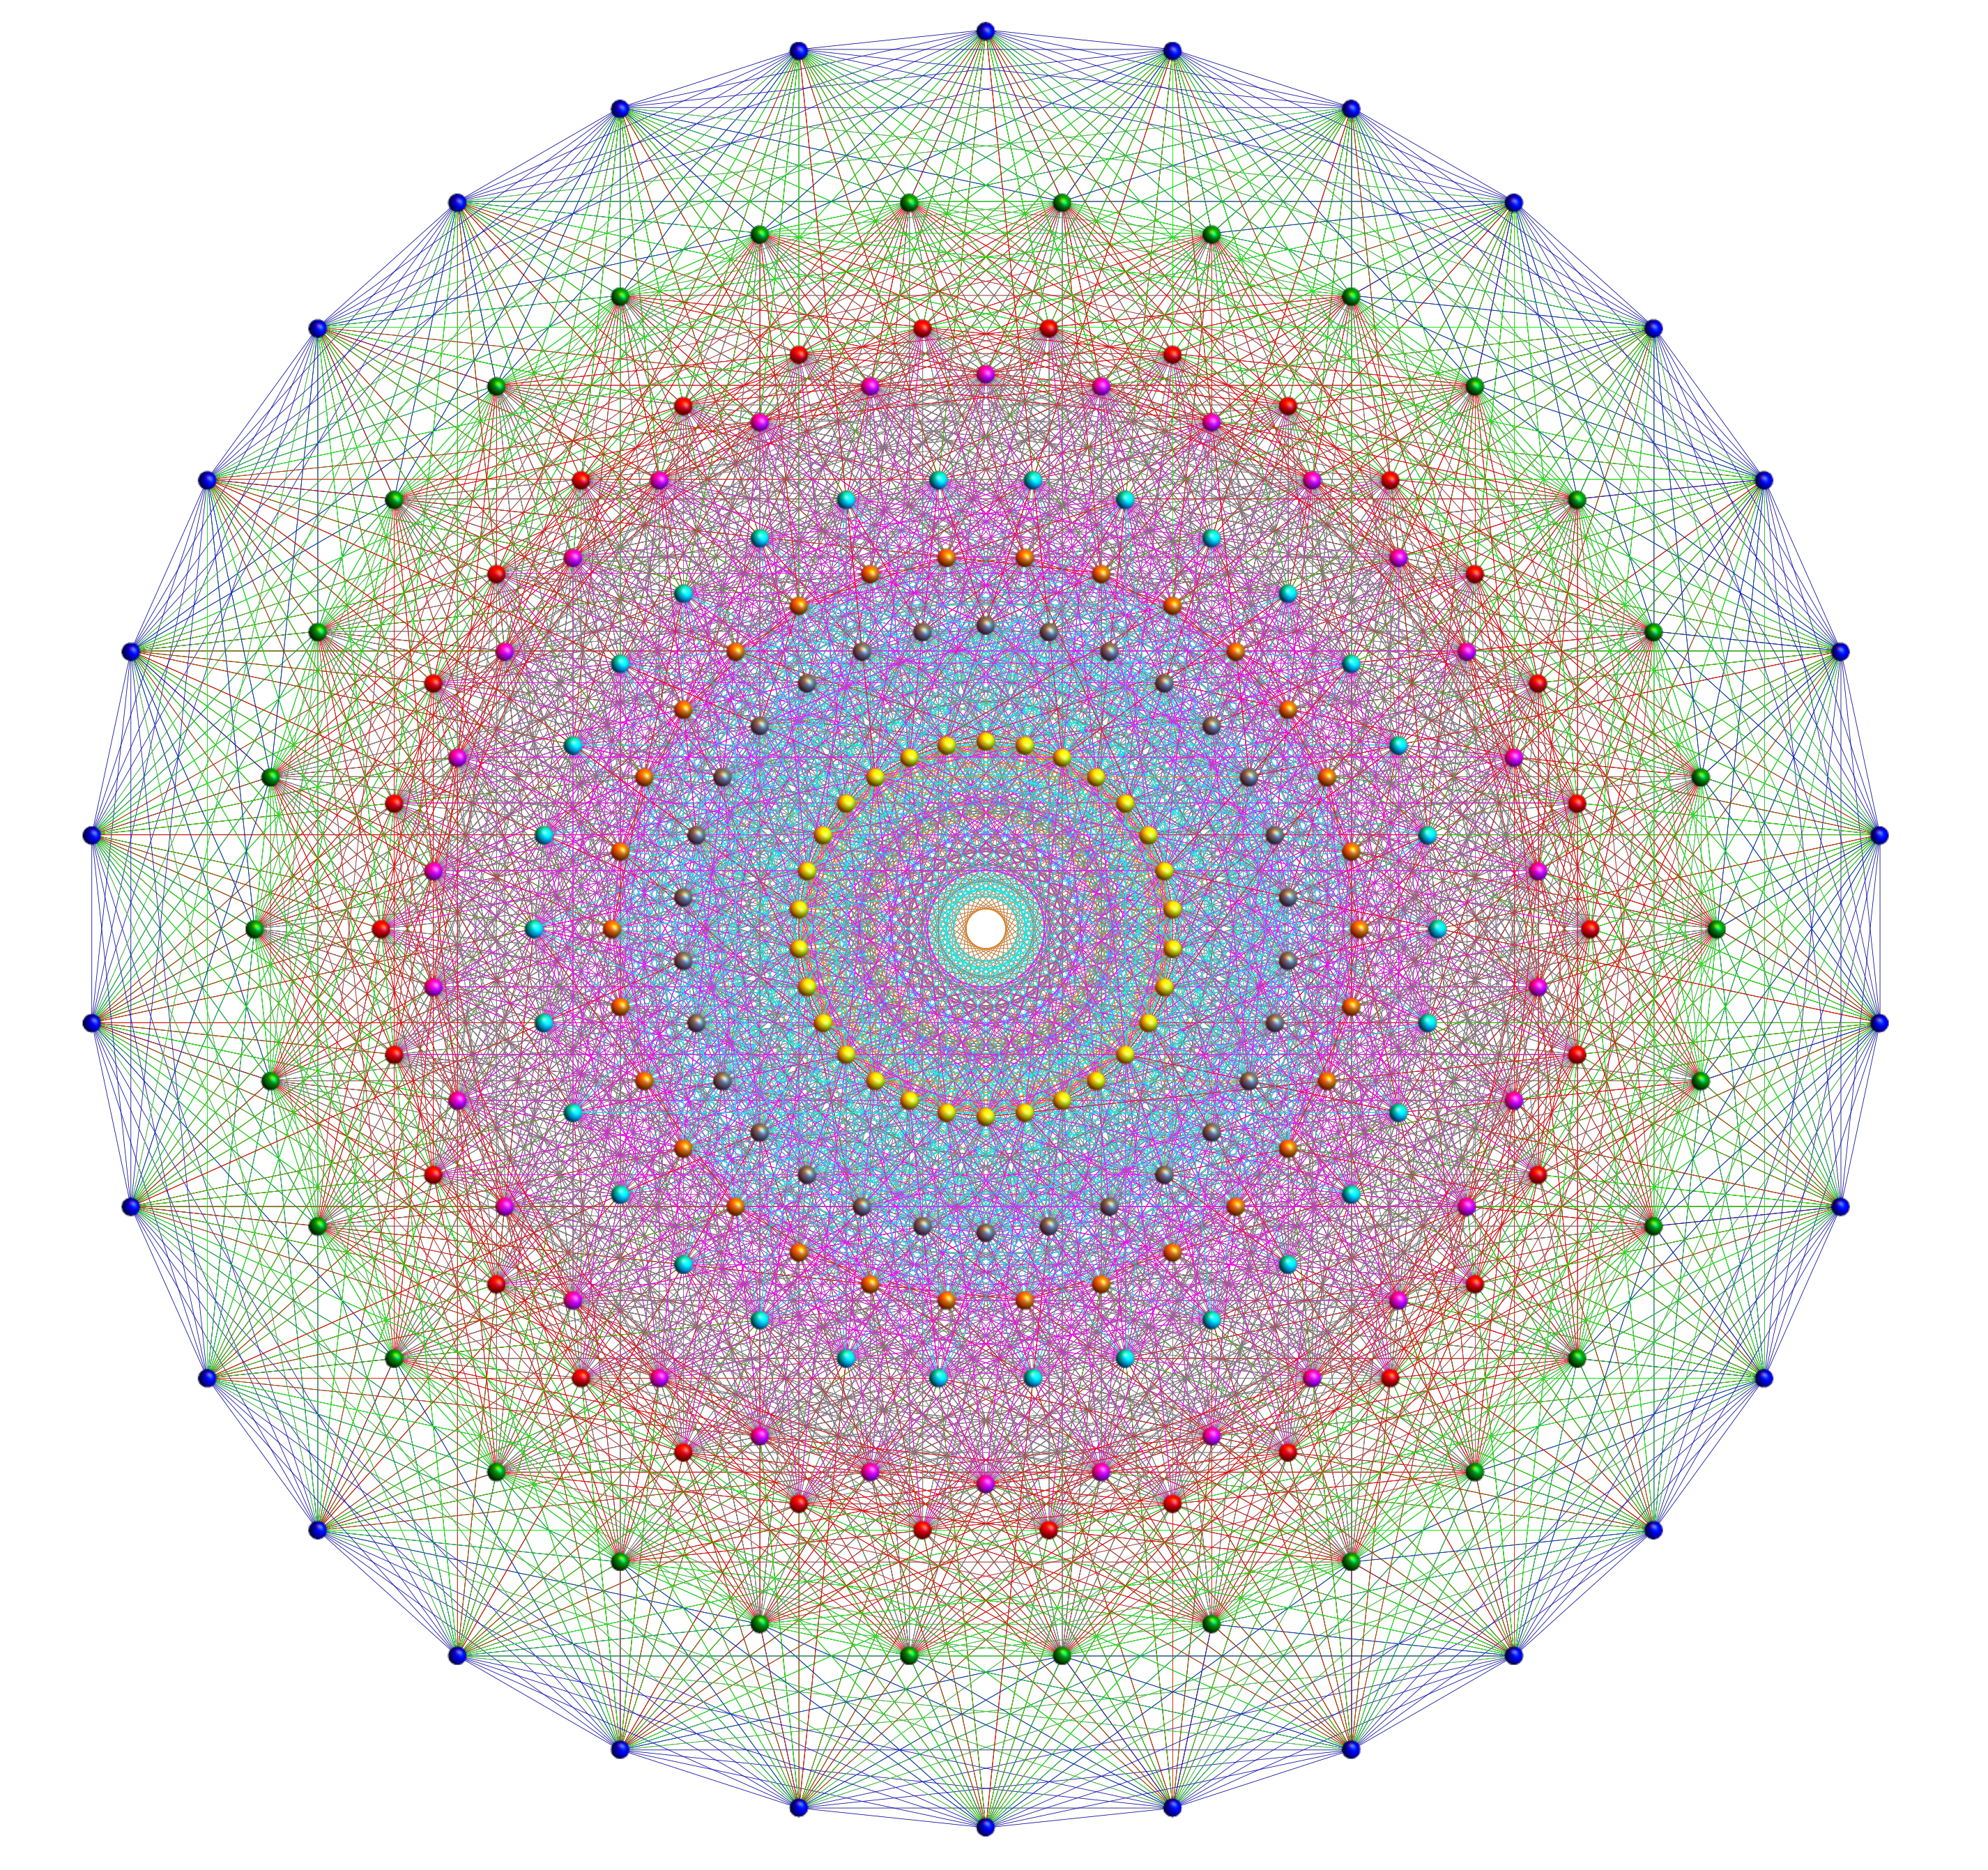
\includegraphics[width=1\columnwidth]{front.png}
\end{figure}
\newpage
\tableofcontents 
\newpage
\section{Gli interi}
\subsection{Propriet\`a di base}
Una propriet\`a dei numeri interi, che si prender\`a come assiomatica, \`e quella del \textit{buon ordinamento}: 
\begin{center}
	\textit{Ogni insieme non-vuoto di interi maggiori o uguali a $0$, ha un elemento minimo.}
\end{center}
Da questa deriva la seguente.
\begin{teorema}
	{Principio di induzione (prima forma)}{}
	Sia $A(n)$ un'affermazione valida per ogni intero $n\ge 1$. Se
	\begin{enumerate}[(1).]
		\item $A(1)$ \`e vera,
		\item $\forall n \ge  1$, se $A(n)$ \`e vera $\implies A(n+1)$ \`e vera,
	\end{enumerate}
	allora, $\forall n \ge  1$, $A(n)$ \`e vera.
	\begin{proof}
		Sia $S $ l'insieme di interi per cui $A(n)$ \`e falsa. Si mostra che $S$ \`e l'insieme vuoto. 
		Si assume per assurdo che $S\neq \varnothing\Rightarrow \exists n_0 \in S$, con $n_0$ minimo (esistente per il buon ordinamento), e, per assunzione, deve essere $n_0 \neq 1 \Rightarrow  n_0>1$. 
		Questo vuol dire che $n_0 -1$ non \`e in $S$ e, quindi, $A(n_0-1)$ \`e vera.

		Per la propriet\`a (2), per\`o, deve essere vera anche $A(n_0)$ perch\'e $n_0 = (n_0-1) + 1$, il che \`e assurdo e, pertanto, $S = \varnothing$.
	\end{proof}
\end{teorema}

\begin{obs}
	Nella dimostrazione sopra, si sarebbe potuto sostituire $1$ con $0$ e far partire il principio di induzione da $n=0$ piuttosto che da $n=1$ e non sarebbe cambiato nulla.
\end{obs}
\noindent Il principio di induzione pu\`o essere espresso in una forma alternativa, come segue.
\begin{teorema}
	{Principio di induzione (seconda forma)}{}
	Sia $A(n)$ affermazione vera $\forall n\ge 0$ e sia possibile mostrare che:
	\begin{enumerate}[(1').]
		\item $A(0)$ \`e vera;
		\item $\forall n > 0$, se $A(k)$ \`e vera $\forall 0\le k < n$, allora $A(n)$ \`e vera.
	\end{enumerate}
	Allora $A(n)$ \`e vera $\forall n\ge 0$.
	\begin{proof}
	Sia ancora $S$ l'insieme degli interi che non soddisfano $A(n)$. 
	Ancora per assurdo, si prende $S\neq \varnothing$, quindi deve esistere, per il buon ordinamento, un $n_0 \in S$ minimo.

	Per punto (1'), deve valere $n_0 \neq 0$ e, visto che $n_0$ \`e minimo, $\forall k$ intero tale che $0\le k< n_0$, $A(k)$ deve essere vera. 
	Per il punto (2'), per\`o, deve essere vera anche $A(n_0)$, arrivando nuovamente all'assurdo.
	\end{proof}
\end{teorema}
\noindent Un altro importante risultato del buon ordinamento \`e l'\textit{algoritmo di Euclide}.
\begin{teorema}
	{Algoritmo di Euclide}{}
	Siano $m,n$ interi, con $m>0$; allora esistono interi $q,r$, con $0\le r< m$, tali che
	\begin{equation}
		n = qm  + r
	\end{equation}
	Inoltre, gli interi $q,r$ sono univocamente determinati da tali condizioni.
	\begin{proof}
		Visto che l'insieme degli interi $q$ tali per cui $qm\le n$ \`e limitato superiormente per definizione, si pu\`o usare il buon ordinamento per affermare che esiste un elemento pi\`u grande\footnote{Basta applicare il buon ordinamento all'elemento più piccolo dell'insieme $n-qm$.} tale che
		\[
		qm \le n < (q+1) m = q m + m
		\] 
		ossia $0\le n - qm < m$. Sia $r = n - qm$, per cui vale $0\le r < m$. Questo dimostra l'esistenza di $r,q$ come descritti.

		Per l'unicit\`a, si assume che valga contemporaneamente
		\[
		\begin{cases}
			n = q_1m + r_1&, \ 0\le r_1<m\\
			n = q_2m + r_2&, \ 0\le r_2<m\\
		\end{cases}
		\] 
		con $r_1 \neq r_2$. Sia, per esempio, $r_2> r_1$; allora, sottraendo le due, si ha $(q_1-q_2) m = r_2-r_1$. 
		Per\`o, si ha $r_2-r_1> 0$ e $r_2-r_1 < m$, il che non \`e possibile perch\'e $q_1-q_2$ \`e un intero per cui $(q_1 - q_2)m > 0$, quindi si avrebbe $r_2-r_1 = (q_1-q_2)m \ge m$ e, quindi $r_2-r_1\ge m$.
		Pertanto, deve essere $r_1=r_2$, che fra l'altro implica $q_1m=q_2m$, per cui $q_1=q_2$.
	\end{proof}
\end{teorema}
\noindent Da questo teorema, si definisce $r$ come il \textit{resto della divisione di $n$ per $m$}.
\subsection{Massimo comune divisore}
Siano $n, d$ due interi diversi da $0$.
Si dice che $d$ \textit{divide} $n$ se esiste $q$ intero tale che $n = dq$; in questo caso, si scrive $d|n$.
Se $m,n$ sono interi non-nulli, per \textit{divisore comune} di $m$ e $n$ si intende un intero $d\neq 0$ tale che $d | m$ e $d | n$. 
Allora si ha la seguente definizione.
\begin{definizione}
	{Massimo comune divisore}{}
	Per massimo comune divisore di $m,n$ interi non nulli, si intende un intero $d>0$, divisore comune di $m$ e $n$, e tale che $\forall e $ intero positivo che divide $m$ e $n$, si ha anche $e|d$.
\end{definizione}
\noindent Chiaramente, il massimo comune divisore \`e univocamente determinato e si mostrer\`a che esiste sempre. 
Per farlo, si d\`a prima la seguente definizione.
\begin{definizione}
	{Ideale}{}
	Sia $J\subseteq \mathbb{Z}$ un sottoinsieme degli interi. Si dice che $J$ \`e un \textit{ideale} se:
	\begin{itemize}
		\item $0 \in J$;
		\item $m,n\in J\implies m+n \in J$
		\item se $m\in J$ e $n$ \`e un intero qualsiasi, allora $mn \in J$.
	\end{itemize}
\end{definizione}
\begin{obs}
	Di seguito, per ideale si intender\`a sempre un sottoinsieme degli interi.
\end{obs}
\noindent Siano $m_1, \ldots,m_r$ interi. Sia $J$ l'insieme di tutti gli interi che si scrivono come
\[
x_1m_1+\ldots+x_r m_r
\] 
con $x_1,\ldots,x_r$ interi. 
Allora \`e automaticamente verificato che $J$ \`e un ideale. Infatti
\begin{itemize}
	\item se $y_1,\ldots,y_r$ sono interi, allora
		\[
		\sum_{i=1}^{r} x_i m_i +  \sum_{j=1}^{r} y_j m_j = (x_1 + y_1) m_1 + \ldots + (x_r + y_r) m_r
		\] 
		che, quindi, appartiene a $J$;
	\item se $n$ \`e un intero, si ha
		\[
		n \sum_{i=1}^{r} x_i m_i = nx_1m_1 + \ldots+ nx_r m_r
		\] 
		che, quindi, appartiene a $J$;
	\item si pu\`o scrivere $0$ come $0m_1 + \ldots + 0m_r$, quindi anche $0 \in J$.
\end{itemize}
In questo caso, si dice che $J$ \`e \textbf{generato} dagli interi $m_1,\ldots,m_r$ e che questi sono i suoi \textbf{generatori}. L'insieme $\left\{ 0 \right\} $ \`e esso stesso un ideale, chiamato \textbf{ideale nullo}. 
Inoltre, $\mathbb{Z}$ \`e detto \textbf{ideale unit\`a}.
Ora si pu\`o dimostrare il seguente.
\begin{teorema}
	{}{smalld}
	Sia $J$ un ideale di $\mathbb{Z}$. Allora esiste un intero $d$ che \`e un generatore di $J$. Inoltre, se $J \neq \left\{ 0 \right\} $, allora $d$ \`e il pi\`u piccolo intero positivo in $J$.
	\begin{proof}
	Sia $J$ l'ideale nullo; allora $0$ \`e un suo generatore.
	Sia, ora, $J \neq \left\{ 0 \right\} $; se $n \in J$, allora $-n = (-1) n $ \`e anche in $J$, quindi $J$ contiene degli interi positivi.
	Si vuole dimostrare che $d$, definito come il pi\`u piccolo intero positivo, \`e un generatore.
	Per farlo, sia $n \in J$, con $n = dq + r, \ 0\le  r < d$; allora $r = n - dq \in J$ e, visto che vale $r < d$, segue che $r = 0$\footnote{Altrimenti $d$ non sarebbe il pi\`u piccolo intero positivo.}, quindi $n = dq$ e, allora, $d$ \`e un generatore.
	\end{proof}
\end{teorema}
\begin{teorema}
	{}{}
	Siano $m_1,m_2$ due interi positivi e sia $d$ un generatore positivo per l'ideale generato da $m_1,m_2$. Allora $d$ \`e il massimo comune divisore di $m_1,m_2$.
	\begin{proof}
		Per definizione, $m_1,m_2 \in J$\footnote{Questo \`e ovvio perch\'e $m_1 = 1m_1 + 0 m_2$ e $m_2  = 0 m_1 + 1 m_2$.}, quindi esiste un intero $q_1$ tale che $m_1=q_1 d$, per cui $d|
		m_1$.
		Analogamente $d|m_2$.
		Sia, poi, $e$ un intero non-nullo che divide sia $m_1$ che $m_2$ come $m_1 = h_1 e$ e $mm_2=h_2 e$, con interi $h_1,h_2$.
		Visto che $d$ \`e nell'ideale generato da $m_1,m_2$, esistono degli interi $s_1,s_2$ tali che $d = s_1m_1 + s_2m_2$, quindi
		\[
		d = s_1h_1e + s_2h_2e = (s_1h_1 + s_2h_2) e
		\] 
		Quindi $e $ divide $d$ e il teorema \`e dimostrato.
	\end{proof}
\end{teorema}
\begin{obs}
	La stessa esatta dimostrazione funziona per pi\`u di due interi, quindi se si considerassero $m_1,\ldots,m _r$ degli interi, con $d$ generatore positivo dell'ideale da loro generato, $d$ sarebbe anche il massimo comune divisore.
\end{obs}
\noindent Questi due teoremi permettono di concludere i seguenti fatti.
\begin{itemize}
	\item Ogni ideale $J$ contiene un numero intero che lo genera interamente e questo coincide col pi\`u piccolo intero positivo in esso contenuto, quindi \`e l'unico generatore \textit{singolo} dell'ideale.
	\item Ogni insieme di numeri interi ha un massimo comune divisore perch\'e tale insieme genera un ideale, il quale, per\`o, contiene un generatore (pi\`u piccolo numero intero in esso contenuto) che \`e un massimo comune divisore per l'insieme di interi iniziale.
\end{itemize}
\begin{definizione}
	{Interi relativamente primi}{relprime}
	Siano $m_1,\ldots,m_r$ degli interi il cui massimo comune divisore \`e $1$. 
	Allora $m_1,\ldots,m_r$ si dicono \textit{relativamente primi} e, per questi, esistono interi $x_1,\ldots,x_r$ tali che
	\[
	x_1m_1   +\ldots + x_r m_r = 1
	\] 
	perch\'e $1$ appartiene all'ideale generato dagli $m_i$.
\end{definizione}
\`E immediato verificare per definizione di ideale che $1 \in  J \iff J \equiv \mathbb{Z}$.
Dalla definizione \ref{def:relprime} segue direttamente che ogni insieme di interi relativamente primi genera $\mathbb{Z}$.
\begin{obs}
	Si potrebbe pensare che se $p$ \`e un numero primo, allora l'insieme $\left\{ p \right\} $ generi $\mathbb{Z}$, cio\`e $p$ generi $\mathbb{Z}$. 
	Questo \`e ovviamente falso sia perch\'e, evidentemente, $J_p$ non contiene $1$, sia perch\'e $p$ non \`e relativamente primo con se stesso, avendo come altro divisore se stesso oltre che $1$.
\end{obs}
\subsection{Fattorizzazione unica}
\begin{definizione}
	{Numero primo}{}
	Si dice che $p$ \`e un numero primo se \`e un intero e $p\ge   2$ tale che, data una fattorizzazione $p = mn $, con interi positivi $m,n$, allora $m=1$ o $n=1$.
\end{definizione}
\begin{obs}
	Il fatto che $p=mn$ con $m=1$, o $n=1$ implica $p$ numero primo significa che $p$ \`e diviso unicamente o da $1$ o, da se stesso.
\end{obs}
\noindent Ora si mostra che ogni numero intero ammette un'unica scomposizione in numeri primi. 
Per dimostrare l'unicit\`a di tale scomposizione, si introduce il seguente lemma.
\begin{lemma}
	{}{lemmaprimdecomp}
	Sia $p$ un numero primo e siano $m,n$ interi non-nulli e tali che $p$ divide $mn$. Allora o $p|m$ o $p |n$.
	\begin{proof}
		Senza perdita di generalit\`a, si assume che $p$ \textit{non} divida $m$. 
		Allora, il massimo comune divisore di $p$ e $m$ deve essere $1$, pertanto esistono interi $a,b$ tali per cui $1 = ap + bm$.

		Ora, moltiplicando ambo i membri per $n$, si ha $n = nap + bmn$, ma $mn = pc$ per qualche intero $c$ (essendo in assunzione $mn$ divisibile per $p$), quindi
		\[
		n = nap + bpc = (na + bc) p
		\] 
		il che implica che $p$ divide $n$.
	\end{proof}
\end{lemma}
\noindent Per evidenziare l'utilit\`a del lemma nel seguente teorema, si nota che se $p$ divide un prodotto di numeri primi $q_1\ldots q_s$, si hanno due possibilit\`a: o $p$ divide $q_1$, o divide $q_2 \ldots q_s$; se divide $q_1$, allora $p \equiv q_1$, altrimenti si trova $p\equiv q_i$ procedendo induttivamente. 
Il caso interessante \`e quando si ha un uguaglianza tra prodotti di numeri primi 
\[
p_1 \ldots p_r = q_1\ldots q_s
\] 
dove ogni $p_i$ divide il prodotto\footnote{Per vederlo, \`e sufficiente prendere $c = p_1 \ldots p_{i-1} p_{i+1} \ldots p_r$, quindi si ha $c p_i = q_1 \ldots q_s$, che \`e la definizione di $p_i | q_1 \ldots q_s$.}. Rinumerandoli, si pu\`o assumere senza perdita di generalit\`a che $p_1 = q_1$ e, induttivamente, che $p_i = q_i$ e $r = s$, essendo due scomposizioni in un numeri primi.
\begin{teorema}
	{}{}
	Ogni intero positivo $n\ge   2$ ammette una fattorizzazione come prodotto di numeri primi (non necessariamente distinti) $n=p_1\ldots p_r$ e tale fattorizzazione \`e unica.
	\begin{proof}
		Si assume per assurdo che esista almeno un intero $\ge  2 $ che non possa essere espresso come prodotto di numeri primi.
		Sia $m$ il pi\`u piccolo di questi. 

		Per costruzione, $m$ non pu\`o essere primo, quindi $m = de$, con $d,e > 1$. 
		Visto che $d$ ed $e$ sono minori di $m$ e visto che $m$ \`e scelto per essere il pi\`u piccolo fra gli interi non fattorizzabili come numeri primi, allora sia $d$ che $e$ ammettono scomposizione in prodotto di numeri primi:
		\[
		\begin{split}
			&d = p_1 \ldots p_r \\
			&e = p'_1 \ldots p'_s
		\end{split}\implies m = p_1 \ldots p_r p'_1 \ldots p'_s
		\] 
	da cui l'assurdo.	

	Per mostrare l'unicit\`a, si usa il lemma \ref{lem:lemmaprimdecomp}. 
	Come conseguenza, diretta del lemma, se esistessero due scomposizioni in primi $p_1 \ldots p_r $ e $p'_1 \ldots p'_s$, varrebbe $p_1 \ldots p_r = p'_1 \ldots p'_s\Rightarrow p_i = p'_i$ e $r = s$, da cui l'unicit\`a
	\end{proof}
\end{teorema}
\subsection{Relazioni di equivalenza e congruenza}
\begin{definizione}
	{Relazione di equivalenza}{}
	Sia $S$ un insieme.
	Una relazione di equivalenza su $S$ \`e una relazione indicata con $x \sim y, \ x, y \in S$, tale che:
	\begin{enumerate}[ER 1.]
		\item $\forall x \in S, \ x \sim x$;
		\item se $x \sim y$ e $y\sim z$, allora $x \sim z$;
		\item se $x\sim y$, allora $y \sim x$.
	\end{enumerate}
\end{definizione}
\noindent Se su $S$ \`e definita una relazione di equivalenza $\sim$, le classi di equivalenza sono insiemi $C_x : = \left\{ y \in S : y \sim x \right\} $ partizionano $S$ in insiemi disgiunti. 
Inoltre, dati due elementi $r,s \in S$, si ha $C_r \equiv C_s$, oppure $C_r,\ C_s$ non hanno elementi in comune.
Si sceglie un elemento che identifica la classe di equivalenza, ad esempio $x$ per $C_x$, e tale elemento si chiama rappresentante della classe di equivalenza. 
Un esempio di relazione di equivalenza \`e la congruenza.
\begin{definizione}
	{Congruenza}{}
	Sia $n$ un intero positivo e siano $x,y$ due interi. Si dice che $x$ \`e \textit{congruente} $y$ \textit{modulo} $n$ se $\exists m : x-y = mn$. In tal caso, si scriver\`a $x \equiv y  \pmod{n}  $.
\end{definizione}
\noindent La congruenza di $x,y$ come $x-y = mn$ implica automaticamente che $x-y$ appartiene all'ideale generato da $n$; inoltre, se $n\neq 0$, allora $x-y$ \`e divisibile per $n$.

Oltre alle propriet\`a delle relazioni di equivalenza, la congruenza ne soddisfa anche altre due:
\begin{itemize}
	\item se $x\equiv y \pmod{n}$ e $z$ \`e un intero, allora $xz \equiv yz \pmod{n}  $;
	\item se $x \equiv y \pmod{n} $ e $x'\equiv y' \pmod{n} $, allora $xx' \equiv yy' \pmod{n} $\footnote{Per dimostrare questa, basta notare che $xx' - yy' = x x' + x'y - x'y - y y ' = x' (x-y) + y ( x'-y')$.} e $x + x' \equiv y + y' \pmod{n} $.
\end{itemize}
Dalla definizione di congruenza, si definiscono gli interi \textbf{pari} come quelli che sono congruenti a $0 \pmod{2} $ (quindi $n = 2m$) e quelli \textbf{dispari} come gli interi che non sono pari, quindi della forma $2m + 1$, per qualche intero $m$.

\newpage

\section{Teoria dei gruppi}

\subsection{Introduzione}

\begin{definizione}
	{Gruppo}{}
	Un \textit{gruppo} $G$ \`e un insieme su cui \`e definita una \textit{legge di composizione} $* : G \to G$ che soddisfa le seguenti condizioni per gli elementi di $G$:
	\begin{enumerate}[GR 1.]
		\item $(x*y) * z =  z*(y * z)$ (\textit{associativit\`a});
		\item $\exists e \in G : x*e = e*x = x$ (elemento neutro);
		\item $\forall x \in G, \ \exists y \in G$ tale che $x*y = y*x = e$ (elemento inverso).
	\end{enumerate}
\end{definizione}
\noindent Quando $*$ \`e la moltiplicazione, $G $ si dice \textbf{gruppo moltiplicativo}; quando $*$ \`e l'addizione, $G $ si dice \textbf{gruppo additivo}.
\begin{definizione}
	{Gruppo commutativo}{}
	Un insieme $G$ \`e detto \textit{gruppo commutativo} se \`e un gruppo e se soddisfa ulteriormente
	\[
	x *y = y *x, \ \forall x,y \in G
	\] 
\end{definizione}
\noindent L'elemento neutro di ciascun gruppo \`e unico.
\begin{proof}
	Sia $e' $ un altro elemento neutro; si nota che: $e = e e' = e'$.
\end{proof}
\noindent L'elemento inverso di ciascun elemento di un gruppo $G$ \`e unico.
\begin{proof}
	Siano $y,y'$ gli elementi inversi di $x$; allora: $e = x y\implies y' e = y' x y \Rightarrow y' = y$.
\end{proof}
\noindent Questo elemento inverso si indica con $x^{-1} $; per gruppo additivo, si indicher\`a con $-x$.
\begin{esempio}
I numeri reali $\mathbb{R}$ e i numeri complessi $\mathbb{C}$ sono entrambi gruppi additivi. I numeri reali diversi da $0$, $\mathbb{R}^*$, e i numeri complessi diversi da $0$, $\mathbb{C}^*$, sono gruppi moltiplicativi.
\end{esempio}
\begin{esempio}
	L'insieme dei numeri complessi di modulo $1$, $\mathscr{I}:= \left\{ z \in \mathbb{C} : |z| = 1 \right\} $, \`e un gruppo moltiplicativo.
\end{esempio}
\begin{definizione}
	{Prodotto diretto}{}
	Siano $G_1, \ldots, G_n$ dei gruppi; si definisce \textit{prodotto diretto} l'insieme
	\[
	G_P = \prod_{i=1} ^n G_i = G_1 \times G_2 \times \ldots \times G_n
	\] 
	e contiene tutte le $n$-uple $(x_1,\ldots,x_n), \ x_i \in G_i$.
\end{definizione}
\noindent Prendendo un prodotto diretto di gruppi ed equipaggiandolo con il prodotto componente per componente, dove l'elemento unit\`a \`e $(e_1,\ldots,e_n)$, con $e_i$ unit\`a di $G_i$, si ottiene un gruppo moltiplicativo.
\begin{definizione}
	{Gruppo finito}{}
	Un gruppo $G$ si dice \textit{finito} se ha un numero limitato di elementi; si chiama \textbf{ordine} il numero di elementi di tale gruppo.
\end{definizione}
\begin{definizione}
	{Sottogruppo}{}
	Sia $G$ un gruppo e $H \subset G$ un sottoinsieme di $G$. Si dice che $H$ \`e un sottogruppo di $G$ se:
	\begin{itemize}
		\item  $e \in H$;
		\item $\forall x,y \in H, \ x*y \in H$;
		\item $\forall x \in H, \ x^{-1}  \in H$.
	\end{itemize}
\end{definizione}
\begin{definizione}
	{Generazione di un sottogruppo}{}
	Sia $S = \left\{ x_1,\ldots,x_n \right\} \subset  G$ un sottoinsieme di un gruppo $G$; l'insieme $H:= \left\{ x \in G : x = x_1 *\ldots*x_n  \right\}\cup \left\{ x^{-1} \in G : x \in S \right\} \cup \left\{ e \in G \right\}  $ \`e un sottogruppo di $G$ ed \`e detto \textit{generato} da $S$, dove gli elementi di $S$ sono detti i \textit{generatori di} $H$.

	In questo caso, si scriver\`a che $H = \langle S \rangle\equiv \langle x_1,\ldots,x_n \rangle$.
\end{definizione}
\begin{esempio}\label{1genz}
Si nota che $\left\{ 1 \right\} $ \`e un generatore per il gruppo additivo degli interi, visto che ogni $z \in \mathbb{Z} \setminus\left\{ 0 \right\} $ si pu\`o scrivere come $1 + 1+ \ldots +1$, o $-1 - 1-\ldots-1$, mentre l'elemento neutro ne fa parte per definizione.
\end{esempio}
Ora si definisce una notazione per indicare una ripetizione dell'operazione di composizione con lo stesso elemento. In generale, si scriver\`a:
\begin{equation}
	x^ n \equiv \underbracket{x *x *\ldots *x}_{n \text{ volte}}
\end{equation}
Se $n=0$, si definisce $x^n = e$; invece, se $n=-m$, si ha la seguente definizione:
\[
x^{-m} = (x^{-1} )^m
\] 
Allora si possono verificare le seguenti:
\begin{itemize}
	\item $x^{n+m} = x^n x^m$;
	\item $x^{-m} x^n = x^{n-m} $;
	\item $(x^n)^m = x^{nm} $.
\end{itemize}
Queste sono direttamente valide per la moltiplicazione, mentre per l'addizione si ha un qualcosa di analogo.
Per cominciare $x^n \equiv nx$ nel caso dell'addizione, per definizione.
Conseguentemente, le regole soddisfatte sono le seguenti:
\[
	(m+n) x = mx + nx \ ; \hspace{.2cm} (mn)x = m(nx)
\] 

Sia, $G$ un gruppo e sia $a \in  G$.
Si definisce il sottogruppo $H$ di $G$ come quell'insieme avente tutti elementi del tipo $a^n, \ \forall n \in \mathbb{Z}$. 
In questo senso, $H$ \`e generato da $a$.
Per mostrare che \`e un gruppo, si nota che :$e \in H$ perch\'e $e = a^ 0 $; dati, poi, $a^n,a^m \in H$, anche $a^{n+m} \equiv a^n a^m \in H $ perch\'e $n+m \in \mathbb{Z}$.
Infine, l'inverso di ciascun elemento $a^n$ appartiene ad $H$ perch\'e $(a^n)^{-1} \equiv a^{-n}  $, che appartiene ad $H$ perch\'e $-n \in \mathbb{Z}$.
\begin{definizione}
	{Gruppo ciclico}{}
	Sia $G$ un gruppo; si dice che $G$ \`e \textit{ciclico} se esiste $a \in G : \forall g \in G, \ g = a^n$, per qualche intero $n$.
\end{definizione}
\noindent Riprendendo l'esempio \ref{1genz}, $\mathbb{Z}$ \`e un gruppo additivo ciclico, con generatore $1$.
Visto che un sottogruppo di $Z$ \`e quello che si \`e chiamato \textit{ideale}, si ha la seguente.
\begin{prop}
	{}{}
	Sia $H$ un sottogruppo di $\mathbb{Z}$. Se $H$ non \`e il sottogruppo banale, sia $d$ il pi\`u piccolo intero in esso contenuto; allora $H$ contiene tutti elementi della forma $nd$, con $n \in \mathbb{Z}$, pertanto $H$ \`e ciclico.
\end{prop}
Sia $G$ un gruppo ciclico e sia $a \in G$ il suo generatore; si hanno due casi possibili.
\begin{itemize}
	\item \textit{Caso 1}: non esiste $n \in \mathbb{Z}^{>0} : a^n = e$.

		Allora per ogni intero $n \neq 0$, $a^n \neq e$ e, allora, $G$ si dice \textbf{infinitamente ciclico}, o che $a$ ha \textbf{ordine infinito} perch\'e ogni elemento $a^n \in G$ \`e distinto dall'altro.
		\begin{proof}
			Si assume $a^r = a^s$ per qualche coppia di interi $r,s$; allora $a^{s-r} = e \Rightarrow s-r = 0 \Rightarrow r=s$.
		\end{proof}
	\item \textit{Caso 2}: $\exists m \in \mathbb{Z}^{>0} : a^m = e$.

		In questo caso, $a$ ha \textbf{ordine finito}. Evidentemente, il gruppo \`e finito perch\'e i suoi elementi si ripetono periodicamente. 

		Sia $J$ l'insieme degli $n \in \mathbb{Z}$ tali che $a^n = e$; allora $J$ \`e un sottogruppo di $\mathbb{Z}$.
		\begin{proof}
			Si ha $0 \in J$ perch\'e $a^0 = e$ per definizione. Se $m,n \in J$, allora $a^{m+n} = a^m a^n = e \Rightarrow  m+n \in J$.
			Infine, visto che $a^{-m} = (a^m)^{-1} =e$, anche $-m \in J$.
		\end{proof}
\end{itemize}
Per il teorema \ref{th:smalld}, il pi\`u piccolo intero positivo contenuto in $J$ genera $J$ stesso;
allora, per definizione, $d$ \`e il pi\`u piccolo intero tale che $a^d = e$ e, per questo, viene chiamato \textbf{periodo} di $a$. 
In quanto tale, se $a^n = e$ per qualche intero $n$, allora $n = ds$, per qualche intero $s$.

\begin{teorema}
	{}{}
	Sia $G$ un gruppo e sia $a \in G$ un elemento di periodo $d$; allora $a$ genera il sottogruppo ciclico di ordine $d$, i cui elementi sono $e, a , \ldots, a^{d-1} $.
	\begin{proof}
	Per mostrare l'esistenza di tale sottogruppo, si nota che per $a \in G$, di periodo $d$, e per generico $n \in \mathbb{Z}$, l'algoritmo euclideo afferma che $n = qd +r $, con $q,r \in \mathbb{Z}$ e $0\le r < d$, per cui vale $a^n = a^r$.

	Ora si mostra che gli elementi sono distinti.
	Se fosse $a^r = a^s$, con $0\le r ,s\le d-1$ e, per assunzione, $r\le s$, allora $a^{s-r} = e $; per\`o $0\le  s-r < d$, quindi bisogna avere $s-r=0$, da cui $r=s$.
	\end{proof}
\end{teorema}
\subsection{Mappe tra gruppi}
Dati $S , S' $ due insiemi, una mappa fra questi \`e indicata con $f: S \to S'$; per $x \in S$, si indica con $f(x) \in S'$ l'immagine di $x$ attraverso la mappa $f$.
Per definire l'immagine di $x$ attraverso $f$, si usa anche la notazione $x \mapsto f(x)$.

Data $f:S \to S'$ e $T \subset S$, si pu\`o definire una mappa che \`e la restrizione di $f$ a $T$, assegnando $x \mapsto f(x), \ \forall x \in T \subset S$; questa si indica con $f|_T : T \to S'$.

Una mappa $f :S\to S'$ si dice \textbf{iniettiva} se $\forall x,y \in S, \ x \neq y \Rightarrow f(x) \neq f(y)$. Una mappa si dice \textbf{suriettiva} se $\forall y \in S', \exists x \in S : f(x) = y $. Infine, $f$ \`e \textbf{biettiva} se \`e sia iniettiva che suriettiva.
Il fatto che $f$ sia biettiva permette di individuare univocamente il suo inverso, la cui esistenza \`e assicurata dalla suriettivit\`a, mentre l'unicit\`a dall'iniettivit\`a.
\begin{definizione}
	{Mappa inclusione}{}
Sia $S$ un insieme e $T \subset S$; la mappa identit\`a di $T$, $\mathrm{id} _T$, vista come mappa $\mathrm{id} _T : T \to S$ \`e chiamata \textit{inclusione} e si indica con il simbolo $T \hookrightarrow S$.
\end{definizione}
\begin{definizione}
	{Composizione}{}
	Date due mappe $f : S \to T, \ g:T \to  U$, si definisce la \textit{mappa composta} come:
	\[
	g \circ f : S \to U , \ (g\circ f ) (x) =  g\big( f(x) \big)
	\] 
\end{definizione}
\noindent Va notato che la composizione \textit{non} \`e commutativa\footnote{se $f(x) = x^2$ e $g(x) = x+1$, si ha $g\circ f = x^2+1$, mentre $f\circ g = (x +1)^2$.}, invece \`e, per definizione, associativa\footnote{Infatti, se $f,g,h$ sono tre mappe tali per cui $h(g(f(x))$ \`e ben definita, allora si ha $h\circ \big(g \circ f\big) = h\circ (g(f(x))=h(g(f(x)))$, ma anche $(h \circ g) \circ f = (h \circ g)\big(f(x)\big) = h(g(f(x)))$.}. 
\begin{prop}
	{}{}
	Siano $S,T,U$ insiemi e siano $f:S \to T , \ g : T \to U$ due mappe; allora:
	\begin{itemize}
		\item $f,g$ iniettive $\Rightarrow g\circ f$ iniettiva;
		\item $f,g$ suriettive $\Rightarrow g\circ f$ suriettiva.
	\end{itemize}
\end{prop}
\begin{definizione}
	{Mappa inversa}{}
	Data $f: S\to S'$ una mappa; la sua inversa \`e la mappa $f^{-1}  : S' \to S$ tale che
	\[
		(f \circ f^{-1} ) (x') = \mathrm{id} _{S'} ; \ (f^{-1} \circ f) (x) = \mathrm{id} _S
	\] 
\end{definizione}
\noindent Indicare l'inversa di $f$ con $f^{-1} $ presuppone che l'inversa sia unica, e infatti \`e cos\`i.
\begin{proof}
	Sia $f:S \to S'$ e siano $g_1, g_2$ due mappe inverse per $f$; ma allora:
	\[
		\mathrm{id} _{S'}(x') = (f\circ g_1) (x') \implies (g_2 \circ \mathrm{id} _{S'}  )(x') \equiv g_2 = g_2\circ (f\circ g_1) = (g_2 \circ f ) \circ g_1 \equiv g_1
	\] 
\end{proof}
\begin{prop}
	{}{}
	Sia $f:S \to S'$; allora $f$ \`e biettiva se e solo se $f$ ha un'inversa.
	\begin{proof}
		Si divide la dimostrazione nelle due implicazioni.
		\begin{itemize}
			\item $(\Rightarrow )$ Si assume che $f$ sia biettiva e si mostra che ha un'inversa.

				La mappa $f$ \`e tale che $\forall x' \in X', \exists ! x \in X : f(x) = x'$; la mappa $x' \mapsto x$ \`e, allora, ben definita e questa coincide con l'inversa.
			\item $(\Leftarrow)$ Si assume che $f$ abbia un'inversa e si mostra che \`e biettiva.

				Per l'iniettivit\`a, si nota che se $x_1\neq x_2 $, allora deve essere anche $x_1' = f(x_1) \neq f(x_2) = x_2'$, altrimenti, se si avesse $f(x_1) = f(x_2) = x'$, $f^{-1} (x')$ non sarebbe una mappa ben definita perch\'e ad un singolo elemento, ne fa corrispondere due.

				Per la suriettivit\`a, il discorso \`e analogo: $f^{-1} :S'\to S$ non sarebbe ben definita se si avesse $x_0' \in S' : \not \exists x \in X , \ f(x) = x_0'$, allora non varrebbe $(f\circ f^{-1} ) (x_0') = \mathrm{id}_{S'}  $.
		\end{itemize}
	\end{proof}
\end{prop}
\noindent Nonostante la precedente proposizione, la notazione $f^{-1} $ si usa anche quando $f:X \to Y$ non ha propriamente un'inversa.
In questo caso, $f^{-1} $ \`e definita come una mappa tra l'insieme dei sottoinsiemi di $Y$ e l'insieme dei sottoinsiemi di $X$.
Cos\`i facendo, si rende possibile avere sempre una $f^{-1} $ perch\'e il suo risultato pu\`o essere l'insieme vuoto (nel caso in cui $f$ non sia suriettiva), oppure un insieme composto da pi\`u elementi nel caso in cui $f$ non sia iniettiva.
\begin{definizione}
	{Permutazione}{}
	Sia $S$ un generico insieme; \`e chiamata \textit{permutazione} di $S$ una mappa biettiva $f: S \to S$ e si indica con $\mathrm{Perm}(S) $ l'insieme delle permutazioni di $S$.
\end{definizione}
\begin{prop}
	{}{}
	L'insieme $\mathrm{Perm} (S)$ \`e un gruppo, la cui legge di composizione \`e data dalla composizione di mappe.
	\begin{proof}
	Si \`e gi\`a mostrato che la composizione di mappe \`e associativa e, chiaramente, esiste la permutazione identit\`a che \`e $\mathrm{id} _S$.

	Inoltre, se $f,g$ sono permutazioni, allora $g\circ f, \ f\circ g : S \to S$ e sono biettive, quindi sono permutazioni. Questo mostra che $\mathrm{Perm} (S)$ \`e chiuso sotto la composizione di mappe.

	Infine, ogni permutazione $f$ ha un'inversa $f^{-1} $ perch\'e $f$ \`e biettiva per definizione.	
	\end{proof}
\end{prop}
\noindent Generalmente, per la composizione di permutazioni, si scrive direttamente $\sigma \tau $, invece di $\sigma \circ \tau $.
\begin{definizione}
	{Sistemi di coordinate}{}
	Siano gli $Y_1,\ldots, Y_n$ degli insiemi; si definisce sistema di coordinate una mappa 
	\[
	f: X \to \prod _{i=1} ^n Y_i = Y_1 \times \ldots \times Y_n, \ f(x) = \big(f_1(x), \ldots, f_n(x)\big)
	\] 
dove $f_i :X \to Y_i, \ i=1, \ldots, n$.
\end{definizione}
\subsection{Omomorfismi, isomorfismi e automorfismi}
\begin{definizione}
	{Omomorfismo}{}
	Dati $G,G'$ due gruppi, un omomorfismo $f: G \to G'$ \`e una mappa che conserva le operazioni di gruppo, cio\`e
	\[
	\forall  x,y \in G, \ f(x*_G y ) = f(x) *_{G'} f(y)
	\] 
	con $*_G, \ *_{G'} $ leggi di composizione, rispettivamente, di $G$ e $G'$.
\end{definizione}
\noindent Si ometteranno i pedici alle leggi di composizioni, ma la distinzione \`e sottintesa.
Per brevit\`a, invece di specificare che in $f:G \to G'$, $G$ e $G'$ sono gruppi, si dir\`a che $f:G\to G'$ \`e un \textit{omomorfismo di gruppi}.
\begin{esempio}
Sia $G$ un gruppo commutativo; allora la mappa $x \mapsto x^{-1} : G \to G $ \`e un omomorfismo. 
Si nota che la richiesta che $G$ sia commutativo \`e fondamentale perch\'e si abbia tale omomorfismo; infatti, $ (x*y)^{-1} = x ^{-1}*y^{-1} $ solamente se $G$ \`e commutativo, altrimenti $x*y *(x*y)^{-1} = e \neq x*y *x^{-1} *y^{-1} $.
\end{esempio}
\begin{esempio}
 La mappa $x\mapsto e^x : (\mathbb{R}, +) \to (\mathbb{R}^{>0} , \cdot )$ \`e un omomorfismo, infatti:
 \[
 x + y \mapsto e^{x+y} = e^x \cdot e^y
 \] 
Questo \`e un esempio in cui le leggi di composizione di gruppo sono diverse perch\'e i due gruppi sono fondamentalmente diversi. 
\end{esempio}
\begin{prop}
	{}{}
	Siano $G,H$ due gruppi, con $H = \prod_{i=1}^n  H_i$. La mappa $f : G \to H $ \`e un omomorfismo se e soltanto se $\forall i, \ f_i$ \`e un omomorfismo.
\end{prop}
\begin{prop}
	{}{}
	Sia $f:G \to G'$ un omomorfismo di gruppi. Allora $f$ conserva l'unit\`a, nel senso che $f(e) = e' $, e conserva l'inversa, nel senso $f(x^{-1} ) = f(x)^{-1} $.
	\begin{proof}
		Per la prima, si nota che $f(e) = f(ee) = f(e)*f(e)$. Moltiplicando (nel senso della legge $*_{G'} $) ambo i membri per $f(e)^{-1} $, si ottiene $e' = f(e)$.

		Per la seconda, sia $x \in G$ tale che $\exists f^{-1} (x)$; allora $e' = f(x*x^{-1} )= f(x) * f(x^{-1} )$. Moltiplicando ambo i membri a sinistra per $f (x)^{-1} $, si ottiene $f (x) ^{-1} = f(x^{-1} )$.
	\end{proof}
\end{prop}
\noindent Si nota che nella proposizione di sopra, si \`e usata la notazione $f(x)^{-1} $ per indicare l'elemento inverso nel gruppo, ossia quell'elemento tale che $f(x) *_{G'} f(x)^{-1} = e'$, ben diverso da $f^{-1} (x)$ funzione inversa, tale che $f \circ f^{-1}=\mathrm{id} $.
\begin{prop}
	{}{}
	Siano $f:G\to G', \ g:G' \to G''$ due omomorfismi di gruppi; allora la loro composizione $g \circ f : G \to G''$ \`e un omomorfismo di gruppi.
	\begin{proof}
		Per calcolo diretto, si ha: $(g\circ f)(x*y) = g\big(f(x*y)\big) = g \big(f(x) * f(y)\big) = g\big(f(x)\big) * g\big(f(y)\big)$.
	\end{proof}
\end{prop}
\begin{prop}
	{}{}
	Dato $f:G \to G'$ un omomorfismo di gruppi, l'immagine di $f$ \`e un sottogruppo di $G'$.
	\begin{proof}
		Dati due elementi $f(x) = x', \ f(y) = y' \in \mathrm{Im} (f) \subset G'$, si ha:
		\[
		x' * y' = f(x) * f(y) = f(x*y) \in \mathrm{Im} (f)
		\] 
		Quindi $\mathrm{Im} (f)$ \`e chiuso rispetto alla legge di composizione definita in $G'$. Anche l'inverso appartiene a $\mathrm{Im} (f)$ perch\'e $x^{-1} \in G \Rightarrow f(x)^{-1} = f(x^{-1} ) \in \mathrm{Im} (f) $. Infine, anche l'identit\`a vi appartiene sempre perch\'e $e \in G \Rightarrow e' = f(e) \in \mathrm{Im} (f)$.
	\end{proof}
\end{prop}
\begin{definizione}
	{Kernel di un omomorfismo}{}
	Sia $f:G \to G'$ un omomorfismo di gruppi; il suo kernel (o nucleo) \`e l'insieme
	\[
	\mathrm{Ker} (f) := \left\{ x \in G : f(x) = e' \in G' \right\} 
	\] 
\end{definizione}
\begin{prop}
	{}{}
	Il kernel di un omomorfismo di gruppi $f:G\to G'$ \`e un sottogruppo di $G$.
	\begin{proof}
		Se $x, y \in \mathrm{Ker} (f)$, allora $x*y \in \mathrm{Ker} (f)$ perch\'e $f(x*y) = f(x) * f(y) = e' * e' = e'$. L'identit\`a appartiene a $\mathrm{Ker} (f)$ perch\'e $f(e) = e'$ e, per finire, se $x \in \mathrm{Ker} (f)$, anche $x^{-1} $ vi appartiene perch\'e $e' = f(e)= f(x * x^{-1} ) = f(x) * f(x^{-1} ) = e' * f(x^{-1} ) \Rightarrow e' = f(x^{-1} )$.
	\end{proof}
\end{prop}
Si considera, ora, un gruppo $G$ e si prende un suo elemento $a \in G$; si nota che la mappa $n\mapsto a^n$ \`e un omomorfismo di $\mathbb{Z}$ in $G$. Questo \`e facile da dimostrare, ma pi\`u interessante \`e il fatto che il kernel di questo omomorfismo pu\`o essere composto o dal solo $0 \in \mathbb{Z}$, o \`e un sottogruppo generato dal periodo di $a$.
\begin{prop}
	{}{}
	Sia $f : G\to G'$ un omomorfismo di gruppi; se $\mathrm{Ker} (f) = \left\{ e \right\} $, allora $f$ \`e iniettivo.
	\begin{proof}
		Si assume, quindi, che $\mathrm{Ker} (f) = \left\{ e \right\} $ e si mostra che $f$ \`e iniettiva. Dati $x,y \in G, \ x\neq y$, se per assurdo, si avesse $f(x) = f(y)$, allora $ e'=  f(x) * f(y)^{-1} = f(x * y^{-1} )\Rightarrow x*y^{-1}  \in \mathrm{Ker} (f)$, con $x*y^{-1}  \neq x * x^{-1} = e$ perch\'e, per assunzione, $x \neq y$.
		Ne segue che $f$ \`e iniettiva.
	\end{proof}
\end{prop}
\noindent Un omomorfismo iniettivo fra due gruppi $G\to G'$ \`e chiamato \textbf{embedding} (o \textbf{iniezione}) e, come l'inclusione, si indica con $G \hookrightarrow G'$.

\begin{prop}
	{}{}
	Sia $f:G \to G'$ un omomorfismo e sia $H' \subset G'$; prendendo $H = f^{-1} (H')$ come l'insieme delle $x \in G : f(x) \in H'$, allora $H$ \`e un sottogruppo di $G$.
\end{prop}
\noindent Si nota che nella proposizione sopra, per $H'=\left\{ e' \right\} $, si ha $f^{-1} (H') \equiv \mathrm{Ker} (f)$.
\begin{definizione}
	{Isomorfismo di gruppi}{}
Dato $f:G\to G'$ un omomorfismo di gruppi, si dice che \`e un \textit{isomorfismo di gruppi} se esiste un altro omomorfismo di gruppi $g : G' \to G$ e tale che $f \circ g = \mathrm{id} _{G'} $ e $ g\circ f = \mathrm{id} _{G} $. 
In tal caso, si dir\`a che $G \approx G'$.
\end{definizione}
\noindent Questo significa che se uno dei due ha delle propriet\`a esprimibili esclusivamente in termini delle operazioni di gruppo, allora anche ogni altro gruppo isomorfo a questo conserva le stesse propriet\`a. 
Alcune di queste sono:
\begin{itemize}
	\item la ciclicit\`a;
	\item l'ordine;
	\item l'essere abeliano.
\end{itemize}
\begin{prop}
	{}{iscond}
	Un omomorfismo di gruppi $f: G \to G'$ che \`e anche biettivo \`e un isomorfismo.
	\begin{proof}
		L'esistenza di $f^{-1} :G' \to G$ \`e assicurata dal fatto che $f$ \`e biettiva. Si deve mostrare che $f^{-1} $ \`e un omomorfismo. 

		Siano dati $x, y \in G': f(x) = x' , \ f(y) = y'\Rightarrow f(x*y) = x'*y'$, visto che $f$ \`e un omomorfismo; allora si nota che:
		\[
		f^{-1} (x'*y')= x*y = f^{-1} (x) * f^{-1} (y) 
		\] 
		
	\end{proof}
\end{prop}
\noindent Dalla precedente proposizione, si ottiene il seguente teorema che permette di capire se un omomorfismo \`e un isomorfismo.
\begin{teorema}
	{}{}
	Sia $f:G \to G'$ un omomorfismo di gruppi. Allora:
	\begin{enumerate}[(a).]
		\item se $\mathrm{Ker} (f) = \left\{ e \right\} \implies f$ \`e un isomorfismo da $G\to f(G) \equiv \mathrm{Im} (f)$;
		\item $f:G\to G'$ \`e suriettiva e $\mathrm{Ker} (f) = \left\{ e \right\} $, allora $f$ \`e un isomorfismo da $G\to G'$.
	\end{enumerate}
	\begin{proof}
		Si \`e gi\`a dimostrato che se il nucleo di $f$ \`e banale, allora $f$ \`e iniettiva; chiaramente $f$ \`e sempre suriettiva dall'insieme di partenza nella sua immagine, quindi la tesi \`e verificata dalla proposizione \ref{prop:iscond}. 

		Sempre per la stessa, segue direttamente il punto (b).
	\end{proof}
\end{teorema}
\begin{definizione}
	{Automorfismo}{}
	Un \textit{automorfismo di gruppi} \`e un isomorfismo $f:G \to G'$ con $G' \equiv G$.
\end{definizione}
\noindent Si indica con $\mathrm{Aut} (G)$ l'insieme di tutti gli automorfismi definiti su $G$. Inoltre, se equipaggiato con la legge di composizione fra funzioni, $\mathrm{Aut} (G)$ \`e un sottogruppo del gruppo delle permutazioni di $G$.
\begin{proof}
	\color{red} DA DIMOSTRARE. 
\end{proof}

\begin{definizione}
	{Traslazione}{}
	Dato un gruppo $G$, la mappa che, per qualche $a \in G$, associa $x \mapsto a*x$, definita da $T_a :G \to G$, \`e chiamata \textit{traslazione}. Questa, in particolare, \`e chiamata traslazione sinistra.
La mappa inversa di una traslazione \`e $T_{a^{-1} } $, in quanto $x = a^{-1} a x$. 
\end{definizione}
\noindent Si consideri la mappa che, per $a \in G$, associa $a \mapsto T_a : G \to \mathrm{Perm} (G)$; questa \`e un omomorfismo perch\'e dati $a, b \in G$, si ha $T_{ab} (x) = abx =( T_a \circ T_b) (x) $, cio\`e $T_{ab} = T_a \circ T_b $.
Evidentemente, questo isomorfismo \`e anche iniettivo perch\'e per $a\neq b$, si ha $T_a \neq T_b$, pertanto $a\mapsto T_a$ risulta un isomorfismo su $G$, la cui immagine non \`e necessariamente coincidente con $\mathrm{Perm} (G)$.
\begin{definizione}
	{Coniugazioni}{}
	Sia $G$ un gruppo e sia $a \in G$; si definisce \textit{coniugazione} la mappa $\mathfrak{c} _a : G \to G$ tale che $x\mapsto axa^{-1} $.
\end{definizione}
\noindent \`E evidente che $\mathfrak{c} _a$ \`e un automorfismo di $G$, in particolare, si definisce \textbf{automorfismo interno}.
La mappa $a \mapsto \mathfrak{c} _a$ \`e un omomorfismo di $G \to \mathrm{Aut} (G)$, la cui legge di composizione \`e la composizione di funzioni.

\begin{definizione}
	{Somma diretta}{}
	Siano $B_1,\ldots,B_r$ dei sottogruppi di un gruppo abeliano additivo $A$; si dice che $A$ \`e \textit{somma diretta} di questi se 
	\[
	A = \bigoplus _{i=1} ^r B_i = B_1\oplus B_2 \oplus \ldots\oplus B_r
	\] 
	cio\`e se $\forall x \in A$, $x = \sum_{i=1}^{r} b_i, \ b_i \in B_i$ \`e scritto \textit{univocamente} come somma di elementi dei $B_i$.
\end{definizione}
\noindent In generale, se $A$ \`e un gruppo additivo abeliano, con $B,  C $ suoi sottogruppi, allora $B+C$ forma un sottogruppo di $A$, i cui elementi sono tutti della forma $b + c, \ b\in B , \ c \in C$.
\begin{teorema}
	{}{}
	Sia $A$ un gruppo abeliano; questo \`e somma diretta di suoi sottogruppi $B, C$ se e soltanto se $A = B+C$ e $B\cap C = \left\{ 0 \right\} $. 
	Questo \`e vero se e soltanto se la mappa $(b,c)\mapsto b+c : B \times C \to A$ \`e un isomorfismo.
\end{teorema}
 Per finire, si considera l'insieme degli omomorfismi tra due gruppi abeliani additivi $A ,B$, indicato con $\mathrm{Hom } (A,B)$. \`E possibile rendere questo un gruppo, definendo $f+g : A \to B$, per $f,g \in \mathrm{Hom} (A,B)$, come
 \[
	 (f+g) (x) = f(x) + g(x), \ \forall x \in A
 \] 
\begin{proof}
	Si mostra che questo, cos\`i definito, \`e un gruppo. Intanto si osserva l'\textit{associativit\`a}:
	\[
	\begin{split}
		&\big( (f+g) + h\big)(x) = (f+g) (x) + h(x) = f(x) + g(x) + h(x)\\
		&\big(f + (g+h)\big)(x) = f(x) + (g+h) (x) = f(x) + g(x) +h(x)
	\end{split}
	\] 
da cui $f + (g+h) = (f+g) +h$. 
Si ha anche l'elemento unit\`a rispetto a $+$, indicato con $0$, che ad ogni elemento di $A$, assegna l'elemento nullo di $B$, che risulta un omomorfismo. 

Per finire, si definisce l'elemento $-f$ con la propriet\`a che $f + (-f) = 0$ e si mostra che $f+g$ e $-f$ sono omomorfismi:
\[
		(f+g) (x+y) = f(x+y) + g(x+y) = f(x) + f(y) + g(x) + g(y) = (f+g) (x) + (f+g) (y)
\] 
e 
\[
	(-f)(x+y) = -\big(f(x+y) \big)= - \big(f(x) + f(y)\big) = - f(x) - f(y)
\] 
Quindi $\mathrm{Hom}(A,B) $ \`e un gruppo.
\end{proof} 

\subsection{Classi laterali e sottogruppi normali}
Siano $S,S'$ due sottoinsiemi di un gruppo $(G,*)$; il loro \textbf{prodotto} \`e:
\begin{equation*}
	S * S' = \left\{ x \in G : x = s * s', \ s \in S,\ s' \in S' \right\} 
\end{equation*}
Allora, se $S_1,S_2,S_3 \subset G$, vale $(S_1 * S_2) * S_3 = S_1 * (S_2 * S_3)$.
Di seguito, alcune altre propriet\`a.
\begin{itemize}
	\item Sia $H$ sottogruppo di $G$; allora $H * H = H$.
		\begin{proof}
			\`E sufficiente prendere l'elemento neutro di uno dei due e far variare tutti gli elementi dell'altro per ottenere tutto $H$. 
			Non si pu\`o uscire da $H$ perch\'e $H$ stesso \`e un gruppo, quindi \`e chiuso rispetto a $*$.
		\end{proof}
	\item Sia $S \subset H$ un generico sottoinsieme e $H$ come sopra; allora $S * H = H$.
		\begin{proof}
			Corrisponde a traslare ciascun elemento di $H$, ma si riottiene comunque $H$. 
			Per vederlo, sia $s \in S$ fissato; dato un generico $h_0 \in H$, si vuole mostrare che $\exists h \in H : s*h= h_0$.

			Visto che $H$ \`e un sottogruppo di $G$, $H$ contiene l'inverso di qualunque suo elemento e di ogni elemento di $S$, pertanto \`e ben definito $h = s^{-1} * h_0$, che soddisfa la richiesta.
		\end{proof}
	\item Dati $S_1,S_2,S_3 \subset G$, allora $S_1 * (S_2 \cup S_3) = S_1*S_2 \cup S_1 * S_3$.
		\begin{proof}
			Si indica con $S: = S_1 * (S_2 \cup S_3)$ e con $\overline{S}:= S_1 * S_2 \cup S_1 * S_3$.

			Un generico elemento di $S$ \`e il prodotto tra $s_1 \in S_1$ e un altro elemento che sta in $S_2$ o in $S_3$.
			Un generico elemento di $\overline{S}$ \`e o il prodotto tra $s_1 \in S_1$ e $s_2 \in  S_2$, o $s_1 \in S_1$ e $s_3 \in S_3$. Allora $S = \overline{S}$.
		\end{proof}
\end{itemize}
\begin{definizione}
	{Classe laterale}{}
	Sia $G$ un gruppo e sia $H$ un suo sottogruppo. Dato $a \in G$, l'insieme di tutti gli elementi della forma $ax, \ x \in H$ \`e chiamato \textit{classe laterale} di $H$ in $G$.

	Si indicher\`a con $aH$.
\end{definizione}
Si nota che, essendo in generale $G$ non-commutativo, la scrittura $aH \neq Ha$; la prima si chiama \textit{classe laterale sinistra}, mentre la seconda sar\`a la \textit{classe laterale destra}.

\begin{obs}
	Pi\`u precisamente dovrebbe essere $a * H$, ma si elimina $*$ per alleggerire la notazione. Nel caso della somma, diventerebbe $a+ H$.
\end{obs}
\begin{teorema}
	{}{}
	Siano $aH$ e $bH$ due classi laterali di $H$ in $G$: o le due classi laterali sono uguali, o non hanno alcun elemento in comune.
	\begin{proof}
		Si assume che $\exists x,y \in H: ax= by$. Allora si osserva che, essendo $xH = H = yH$:
		\[
		aH = axH = byH = bH
		\] 
	\end{proof}
\end{teorema}
\`E possibile decomporre un gruppo in classi laterali. 
Si considera il caso specifico di $G$ grupp[o finito; ogni elemento $x \in G$ appartiene ad una classe laterale, per esempio $xH$, con $H$ sottogruppo di $G$.
Allora, $G$ si pu\`o scrivere come unione finita di classi laterali di $H$:
\begin{equation}
	G = \bigcup_{i=1} ^r a _i H
\end{equation}
dove ogni classe laterale \`e distinta dall'altra, altrimenti sarebbero uguali e non si sarebbe aggiunto nessun nuovo elemento di $G$.
Ogni elemento $ah, \ h \in H$ \`e chiamato \textbf{rappresentante} della classe laterale $aH$.

Lo stesso si pu\`o dire per gruppi infiniti, ma sono ammesse unioni di infinite classi laterali; indicando con $I$ un certo insieme di indicizzazione potenzialmente infinito:
\begin{equation}
	G = \bigcup _{i \in I} a _i H
\end{equation}
con $G$ finito o infinito.
\begin{teorema}
	{}{}
	Sia $G$ un gruppo e $H$ un sottogruppo finito. Allora il numero di elementi di una certa classe laterale $aH$ \`e il numero di elementi di $H$.
\end{teorema}
Dati $G,H$ come al solito, si indica con $G/H$ l'insieme di tutte le classi laterali sinistre di $H$ in $G$.
Si chiama \textbf{indice} il numero di tutte le distinte classi laterali di $H$ in $G$ e si indica con $(G:H)$.
Se $\# S$ \`e il numero di elementi in $S$, allora $\# (G / H) = (G:H)$ e $\# G = (G:1)$.
\begin{teorema}
	{}{}
	Sia $G$ un gruppo finito e $H$ un suo sottogruppo. Allora:
	\begin{enumerate}[(a).]
		\item $\mathrm{ord}(G) =  (G:H) \cdot \mathrm{ord} (H) $, con $\mathrm{ord} (\cdot )$ che indica l'ordine di un certo gruppo finito;
		\item dato $L \subset G$ un generico sottogruppo, $\mathrm{ord}(L) $ divide $\mathrm{ord}(G) $;
		\item dato $a \in G$, il periodo di $a$ divide $\mathrm{ord}(G) $;
		\item se $G \supset H \supset K$ sono sottogruppi, allora $(G:K) = (G:H)(H:K)$.
	\end{enumerate}
\end{teorema}









\end{document}
